% ==========================================================================
% ======================== Dokumentace k PC 1.0 ;-) ========================
% ==========================================================================

% Ověřeno, prošlo bez jediné připomínky - při dodržení následujících pokynů:
% - SPRÁVNĚ vyplnit titulní stranu (!!!)
% - Nadpisy používat v pořadí (zanoření):
% 		- chapter (celá kapitola)
%		- section
% 		- subsection, subsubsection ... 
% - Pro pomlčky V TEXTU používat -- (doslova 2 mínusy). Neplatí pro rozsahy
%	(0-9), spojovníky typu xxx-li apod.
% - Uvozovky - používat české \uv{hezké uvozovky}.
% - Zvýrazňovat \textit{kurzívou}.
% - Názvy modulů, funkcí psát \texttt{neproporcionálním fontem}.
% - URL psát do \url{}
% - In-line matematické výrazy přímo do řádky $uzavřené do dolarů$, složitější
%	na samostatnou řádku $$do dvojitých$$.
% - Pokud např. v zadání zmiňujete LATEX a TEX, použít \latex resp. \tex.

% - Pozor na předložky a spojky - nesmí se vyskytovat na konci řádku => použít
%	nedělitelnou mezeru (~).
% - Nové odstavce dvojitým odřádkováním.

% OBRÁZKY	- Vektorově (!!!) - Illustrator, free Inkscape.
% 			- Rastrově vkládat jen screeny obrazovky.
%			- V textu pak odkazovat pomocí \ref{img1}.
%			- Pro úpravu velikosti změnit scale.
% 	\begin{figure}[h]
%		\centering
%		\includegraphics[scale=1.0]{soubor.pdf/png}
%		\caption{Popisek}
%		\label{img1}
%	\end{figure}

% PŘELOŽENÍ
% - Nainstalovat doporučený MiKTeX.
% - "pdflatex <nazev-souboru>.tex"
% - Pro správné vygenerování odkazů, obsahu nutné vždy spustit 2x (!!!)
% - Pro zjednodušení stačí spouštět přibalený bat, který to udělá sám ;)

% ^^^^^^^^^^^^^^^^^^^^^^^^^^^^^^^^^^^^^^^^^^^^^^^^^^^^^^^^^^^^^^^^^^^^^^^^^^
% ^^^^^^^^^^^^^^^^^ !!!!!!!!!SMAZAT PŘI ODEVZDÁNÍ!!!!!!!!! ^^^^^^^^^^^^^^^^^
% ^^^^^^^^^^^^^^^^^^^^^^^^^^^^^^^^^^^^^^^^^^^^^^^^^^^^^^^^^^^^^^^^^^^^^^^^^^

\documentclass[
12pt,
a4paper,
pdftex,
czech,
titlepage
]{report}

\usepackage[czech]{babel}
\usepackage[utf8]{inputenc}
\usepackage{lmodern}
\usepackage{textcomp}
\usepackage[T1]{fontenc}
\usepackage{amsfonts}
\usepackage{titlesec}
\usepackage{graphicx}
\usepackage[hidelinks]{hyperref}
\usepackage{caption}
\usepackage{pdfpages}
\usepackage{xcolor}

\usepackage{listings}
\usepackage{mips}


\titleformat{\chapter}
  {\normalfont\LARGE\bfseries}{\thechapter}{1em}{}
\titlespacing*{\chapter}{0pt}{0ex plus 1ex minus .2ex}{2.0ex plus .2ex}

\begin{document}

\begin{titlepage}
	\vspace*{-2cm}
	{\centering
\includegraphics[scale=0.5]{FAV_logo_jvs}\par}
	\centering
	\vspace*{2cm}
	{\Large Semestrální práce z KIV/UPA\par}
	\vspace{1.5cm}
	{\Huge\bfseries MIPS\par}
	\vspace{2cm}

	{\Large Petr Laštovka\par}
	{\Large A15B0055K\par}
	{\Large jokertwo@students.zcu.cz\par}

	\vfill

	{\Large 25.\,1.\,2019}
\end{titlepage}

\thispagestyle{empty}
\clearpage


% Table generated by Excel2LaTeX from sheet 'Sheet1'
\chapter{Zadání}
Naprogramujte jednoduchý program pro výpočet obsahu trojúhelníka. Trojúhelník bude zadán třemi body. Vstup bude zadáván z klávesnice a výstup na obrazovku ve vhodném formátu.

\chapter{Analýza}
 Pro výpočet obsahu trojúhelníka bude využit vektorový součin a vzorec pro výpočet obsahu rovnoběžníku. 
 
 \section{Vektorový součin}
 U vektorového součinu je výsledkem vektor, který je kolmý na oba předešlé vektory. Vektorový součin vektorů $u$, $v$ se značí: $u \times v$ 
$$ u \times v = (u_2v_3-u_3v_2; u_3v_1-u_1v_3; u_1v_2-u_2v_1)$$

 \section{Význam vektorového součinu}
Kromě toho, že pomocí vektorového součinu určíme vektor kolmý na oba původní vektory (čehož využijeme například přu určování obecné rovnice roviny), můžeme také spočítat obsah rovnoběžníku daného původními vektory:

\begin{figure}[h]
	\centering
	
		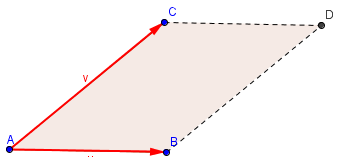
\includegraphics[scale=.5]{404.png}
		\caption{Rovnoběžník}
		\label{fig:klient01}
	\end{figure} 

Obsah rovnoběžníku $ABCD$ z předchozího obrázku by se spočítal jako velikost vektorového součinu:
$$u = B - A $$
$$v = C - A $$
$$S = |u \times v |$$

Vektorovým součinem dokážeme spočítat obsah rovnoběžníku a zárovnň platí, že složíme-li dva stejné trojúhelníky vedle sebe, vznikne rovnoběžník. Pokud tedy spočítáme obsah rovnoběžníku daného vektory $u, v$ a vydělíme ho dvěma, získáme obsah trojúhelníku $ABC$.

\chapter{Program}
\lstset{language=[mips]Assembler}
\begin{lstlisting}
   .data
	souTextA0: .asciiz "Zadejte souradnici A[0]:\n"
	souTextA1: .asciiz "Zadejte souradnici A[1]:\n"

	souTextB0: .asciiz "Zadejte souradnici B[0]:\n"
	souTextB1: .asciiz "Zadejte souradnici B[1]:\n"

	souTextC0: .asciiz "Zadejte souradnici C[0]:\n"
	souTextC1: .asciiz "Zadejte souradnici C[1]:\n"	
	
	vysledek: .asciiz "Obsah trojuhelniku je: "
	
	half: .float 2.0
	
	.text
	.globl main
	
main:	
	########  nacteni uzivatelskeho vstupu ##########
	la $a0,souTextA0	# argument: string
	jal nactiCislo		# procedura pro nacteni
				# vtupu od uzivatele
	la $a0,souTextA1	# argument: string	
	
	jal nactiCislo		# procedura pro nacteni
				# vtupu od uzivatele
	move $t0,$v0		# ulozeni 1. vstupu
				# od uzivatele
	la $a0,souTextB0	# argument: string
	move $t1,$v0		# ulozeni 2. vstupu
				# od uzivatele
			
	jal nactiCislo		# procedura pro nacteni
				# vtupu od uzivatele
	la $a0,souTextB1	# argument: string
		
	jal nactiCislo		# procedura pro nacteni
				# vtupu od uzivatele
	move $t2,$v0		# ulozeni 3. vstupu
				# od uzivatele		
	la $a0,souTextC0	# argument: string
	move $t3,$v0		# ulozeni 4. vstupu
				# od uzivatele	
	
	jal nactiCislo		# procedura pro nacteni
				# vtupu od uzivatele
	la $a0,souTextC1	# argument: string
	jal nactiCislo		# procedura pro nacteni
				# vtupu od uzivatele
	move $t4,$v0		# ulozeni 5. vstupu
				# od uzivatele
	move $t5,$v0		# ulozeni 6. vstupu
				# od uzivatele

	########   vypocteni vectoru U ########  
		
	sub $t6,$t2,$t0		
	sub $t7,$t3,$t1
	
	########  vypocteni vectoru V########  
	
	sub $t8,$t4,$t0
	sub $t9,$t5,$t1
	 	
  	########  nasobeni vektoru U x V ########  
  	
  	mul $v0,$t6,$t9
	mul $v1,$t7,$t8
  	
  	
  	sub $t6,$v0,$v1
  	ble $t6,$zero,normalizace
  	j deleni

deleni:		nop
		lwc1 $f2,half		# ulozi do $f2 hodnotu 2
		mtc1 $t6,$f0		# ulozi obsah $t6
				# do coprocesoru na adresu $f0
		cvt.s.w $f0,$f0		# prevede integer na float
  		div.s $f12,$f0,$f2	# vydeli dva floaty
  		j tiskVysledek		# pokracovani na proceduru
				# ktera vytiskne vysledek
  		
tiskVysledek:	nop
		la $a0,vysledek		# nacteni string retezce
		li $v0,4		# syscall 4 (print_str)
		syscall			# zavolani syscall

		li $v0,2		# syscall 2 (print_float)
		syscall			# zavolani syscall
		j exit
 
nactiCislo: 	nop
		li $v0,4		# syscall 4 (print_str)
		syscall			# zavolani syscall
		
		li $v0,5		# sluzba nacti cislo
		syscall			# zavolani syscall
		jr $ra			# navrat z procedury
		
normalizace: 	nop			
		mul $t6,$t6,-1		# pronasobi cislo
				# -1 k dostani kladneho cisla
		j deleni		# pokracovani ve vypoctu

exit: 		nop
		li $v0,10		# oznameni systemu
				# ze program bude koncit
		syscall			# syscall

\end{lstlisting}

\chapter{Vstup a výstup programu}
Veškeré vstupy a výstupy do programu se provádí prostřednictvím konzole.
\section{Vstup}
Po spuštení programu je uživatel vyzván aby postupně zadávál jednotlivé souřednice troujúhelníku (viz obr \ref{fig:klient01})

\section{Výstup}

Výstupem programu je informování uživatele o obsahu trojúhelníka. Ukázka možného výstupu obr \ref{fig:klient01}.

\begin{figure}[h]
	\centering
	
		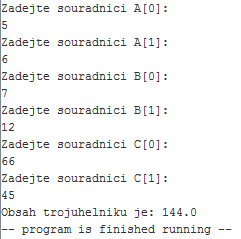
\includegraphics[scale=1]{45.PNG}
		\caption{Vstup a výstup programu}
		\label{fig:klient01}
	\end{figure} 
	
\chapter{Závěr}
Práci jsem vypracoval v programu MARS 4.5. Tento program má uživatelsky přívětivé prostředí a snadno se v něm sleduje běh programu. Naneštěstí tento program neumožnuje simulovat zpožděné načítání. Z toho důvodu jsem výslednou aplikaci odladil na programu QtSpim tak aby vyhovovala zadání. \par
Úlohu jsem vypracoval tak aby program využíval zpožděné skoky a zpožděné načítaní ve svůj prospěch a optimalizaci. Během psaní programu jsem se seznámil s architekturou MIPS a s problémy zpožděných skoků a načítání.
	
\begin{thebibliography}{0}
\bibitem{bib.modelovani}Analytická geometrie - Vektorový součin, https://maths.cz/clanky/107-analyticka-geometrie-vektorovy-soucin ,on-line
\end{thebibliography}
\end{document} 